\documentclass[11pt]{article}
    \usepackage{amsmath}
    \usepackage[pdftex]{graphicx}
    %\usepackage[usenames,dvipsnames,svgnames,table]{xcolor}
    \usepackage{amsmath,amsthm,amssymb,color,wrapfig,floatflt,amsfonts,listings,fancyhdr}
    \usepackage[parfill]{parskip}
    %\pagestyle{plain}
    \setlength\topmargin{.1cm}
    %\setlength\textheight{8in}
    \setlength\oddsidemargin{.1in}
    \setlength\evensidemargin{.1in}
    \setlength\textwidth{6.51in}
    %\setlength\headheight{52.5pt}
    \usepackage{fancyhdr}
    \usepackage[algosection, boxruled, linesnumbered]{algorithm2e}
    \pagestyle{fancy}
    \lhead{Arvind Ramaswami}
    \rhead{HW4}
    \chead{CS 4641 Machine Learning}
    \lfoot{}
    \cfoot{Page {\thepage}}
    \rfoot{}
    \newcommand{\RR}{\mathbb{R}}
    \newcommand{\CC}{\mathbb{C}}
    \newcommand{\HH}{\mathbb{H}}
    \newcommand{\BB}{\mathbb{B}}
    \newcommand{\ZZ}{\mathbb{Z}}
    \newcommand{\QQ}{\mathbb{Q}}
    \newcommand{\NN}{\mathbb{N}}
    \newcommand{\cP}{\mathcal{P}}
    \renewcommand{\And}{\wedge}
    \newcommand{\Or}{\vee}
    \newcommand{\Implies}{\Rightarrow}
    \newcommand{\Not}{\sim}
    \begin{document}
        \section{Introduction}
            
            This project investigates the use of different MDP and reinforcement learning
            algorithms to solve MDP problems.

            \subsection{MDP problems}

            Both of the MDP problems are variants of a maze problem. This is a rectangular board
            with multiple tiles, and from a certain tile $s$, the agent can choose to move
            up, down, left, or right. When choosing an action $a$ from state $s$, the agent
            will move to some state $s'$ with a transition probability $T(s, a, s')$. The
            goal is to find an optimal state-to-action mapping such that the expected reward
            is maximized over several states.

            There are walls on the grid, and bumping into them produces a penalty of 50 (
            for the sake of this MDP problem, this can be interpreted as a gain of -50
            reward
            ). Thus, a way to think of this problem is that we want to maximize reward
            by minimizing the number of walls that are bumped into.
            
            One of the problems is a maze on a 10 x 10 grid, and the other one is
            a maze on a 70 x 70 grid. For the purposes of these experiments, %change to larger state space?
            this maze problem is interesting, since the two-dimensional state space allows the
            optimal action from each state to be readable to the human eye. Thus,
            the arrangement of the states in gridworld allows one to effectively tell
            how well one algorithm is doing compared to the other just by eyeballing the
            actions at every state.

            Many well-known MDP's like GridWorld involve maximizing some positive
            amount of expected reward, but it is interesting that reinforcement can
            alternatively be applied for cost-minimization problems (in this case
            minimizing the number of walls that are bumped into).
            
            


            \subsection{Experiments}
            
            The actions in these experiments have some stochastisity, given a state and action, there is a 70 percent change
            that the agent will travel to the intended state and a 30 percent chance that the agent will travel to another
            random state. In the RL-MDP simulation, this feature is controlled by the value of the PJOG parameter,
            which is set to .3 (which means there is a 1 - .3 = .7
            chance of the agent going in the intended direction).

           
        \section{Results and Analysis}

        Below are some screenshots of the running of the various experiments.
        At each tile, there is a line segment, with one endpoint at the center
        of the tile and the other endpoint in another direction. The direction
        of each segment at each tile represents the optimal action to
        take from that particular state. Also, there is a number on each
        tile, which is proportional to the expected utility that would occur
        if the particular policy is chosen.

        \subsection{Maze: Fewer States}

            Here is the image of the particular maze that was used for the
            experiment with fewer states:

            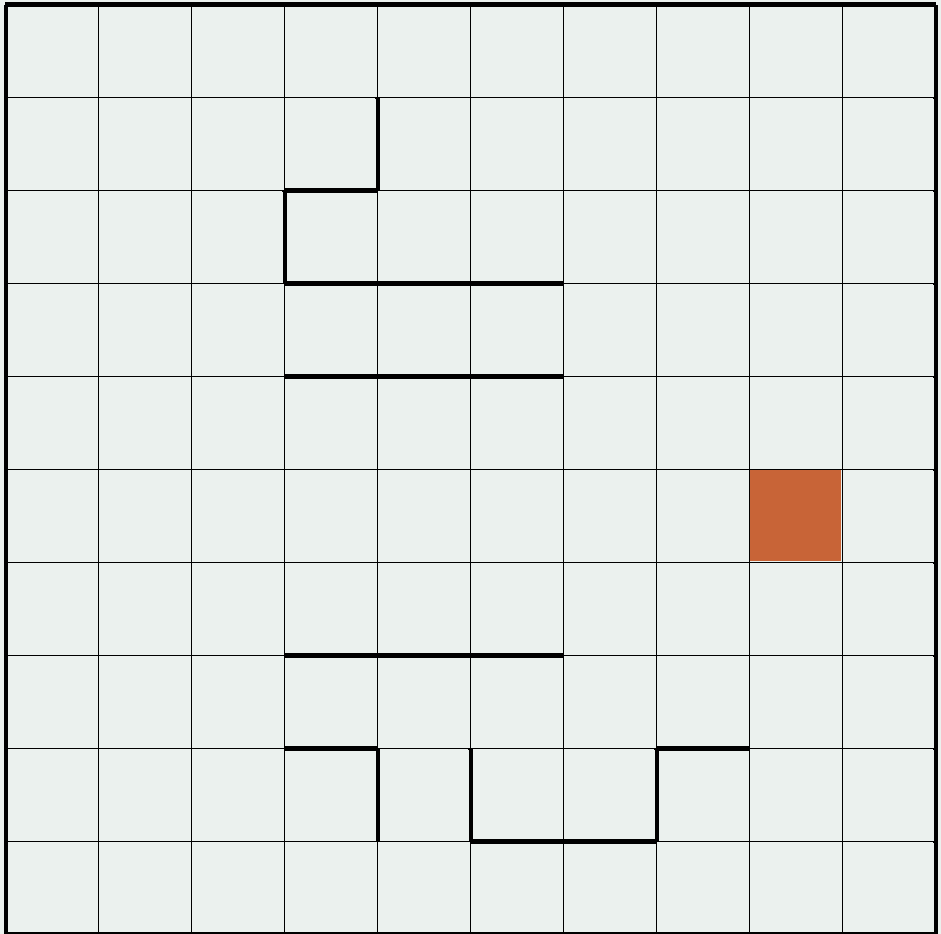
\includegraphics[width=5cm]{../images/small/maze.PNG}

            \subsubsection{Value iteration}

            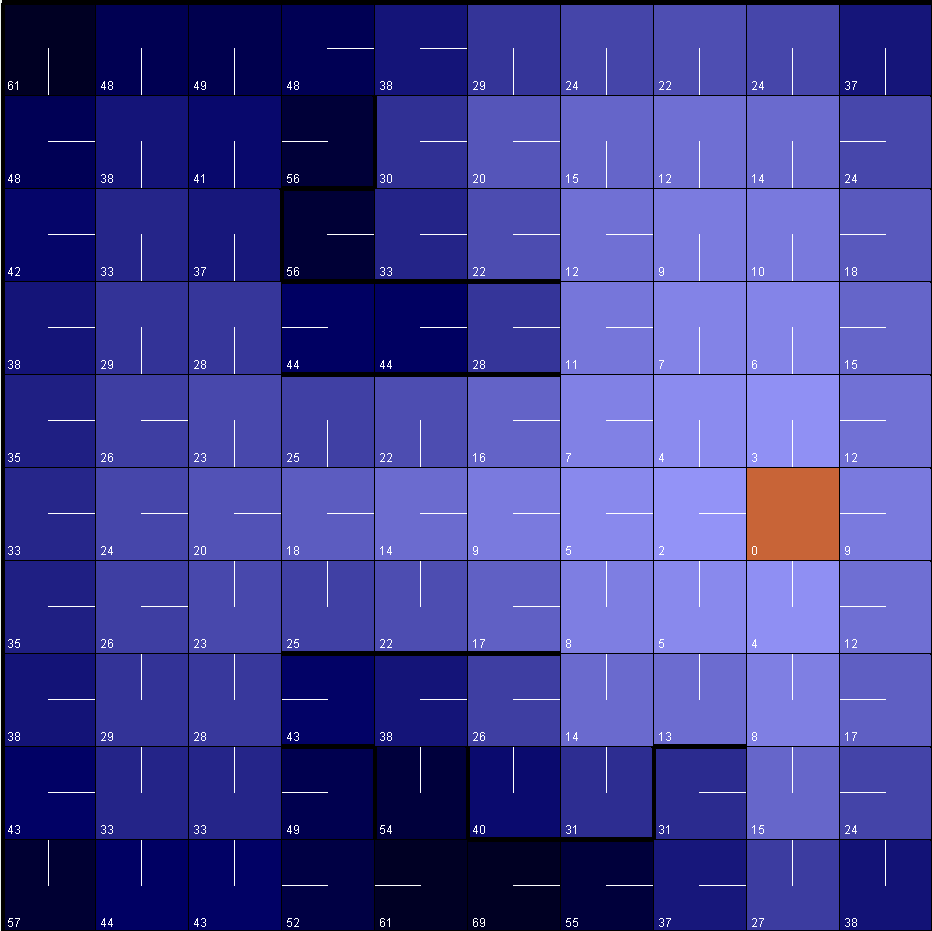
\includegraphics[width=5cm]{../images/small/vi.PNG}

            With a precision parameter of 0.001, PJOG = 0.3,
            and wall penalty of 50, this algorithm took 61 steps
            to converge, taking a total of 69 ms.

            \subsubsection{Policy Iteration}

            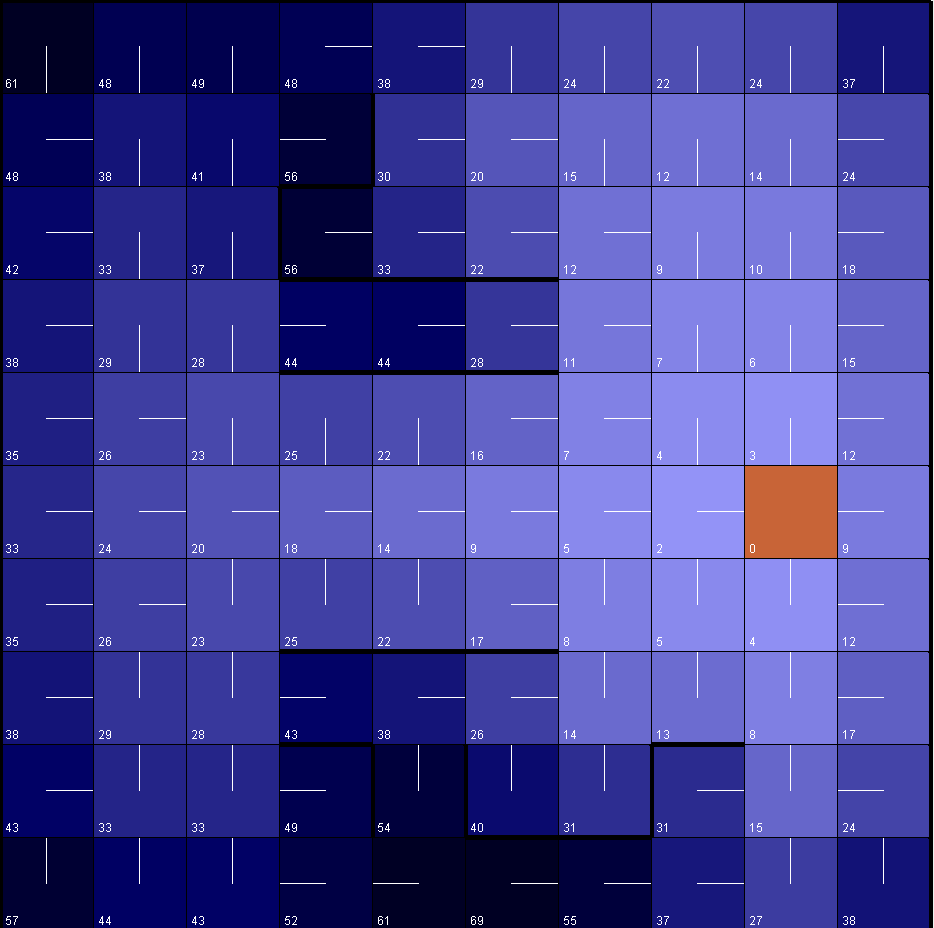
\includegraphics[width=5cm]{../images/small/pi.PNG}

            The iter. limit parameter (the maximum number
            of times for the policy to be evaluated) was set
            to 10, and the value limit (the maximum number of
            value updates within each policy iteration) was
            set to 5000. The algorithm converged within 6 policy
            evaluation iterations, taking a total of 19 ms.


            Here, policy evaluation worked more quickly than value iteration and
            still gave similar result on the maze tile values. Of course, each
            policy iteration took much longer than each value iteration,
            since the number of steps in the algorithm was equal to $S^2 * 10$,
            but there were much fewer iterations in the policy iteration algorithm.

            For each state in each value iteration, the algorithm needed to consider
            what the expected utility by moving up, down, left, or right. This was
            unlike what happened in policy iteration, where the algorithm only considered
            the result of one action, allowing for fewer computations.
            
            Also, each value iteration involved observing what happens when moving either direction only once,
            while policy iteration involved observing what happens when moving in a fixed direction several times.
            This made the value iteration algorithm more prone to noise from taking each action
            from a state, since each action is taken only once; since policy iteration takes that fixed action
            ten times from that state, it is able to disregard stochastic irregularities for a particular
            action.

            The policy iteration experiment discussed here mentions a 53 ms run that is caused by
            10 inner iterations in policy evaluation. However, this can be sped up even more by
            decreasing the number of inner iterations. The total number of policy iterations doesn't
            increase here, since the expected number of tiles that random noise would affect is
            smaller with this small maze state.

            The faster time for fewer inner policy iterations and the fixed number of total policy
            iterations can be confirmed by the table below (which measures policy iterations
            and time for varying numbers of inner iterations):

            \begin{tabular}{c c c}
                Inner iterations & Policy iterations & Time \\ \hline
                1 & 6 & 4ms \\ \hline
                2 & 8 & 8ms \\ \hline
                5 & 8 & 12ms \\ \hline
                10 & 6 & 19ms \\ \hline

            \end{tabular}


            \subsubsection{RL}

            On this MDP, Q-learning was done for 1000 episodes. The learning
            rate was set to 0.7, and it was made such that it decays.

            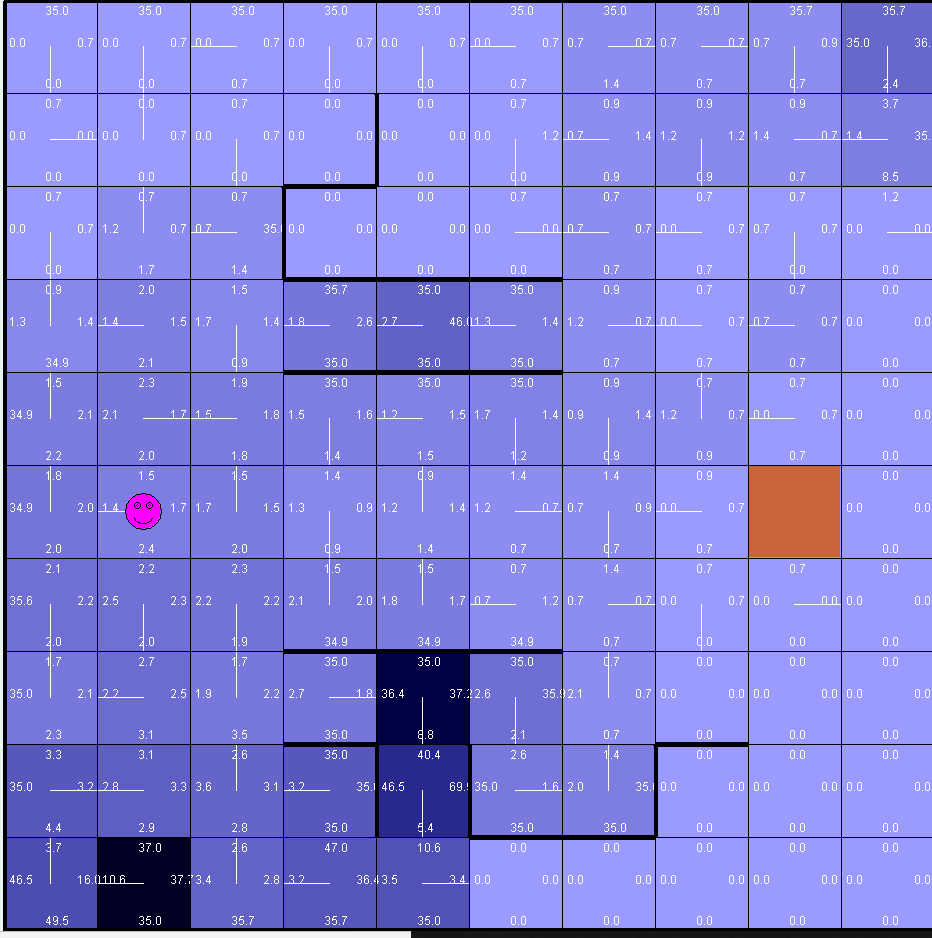
\includegraphics[width=5cm]{../images/small/q_middle.PNG}
            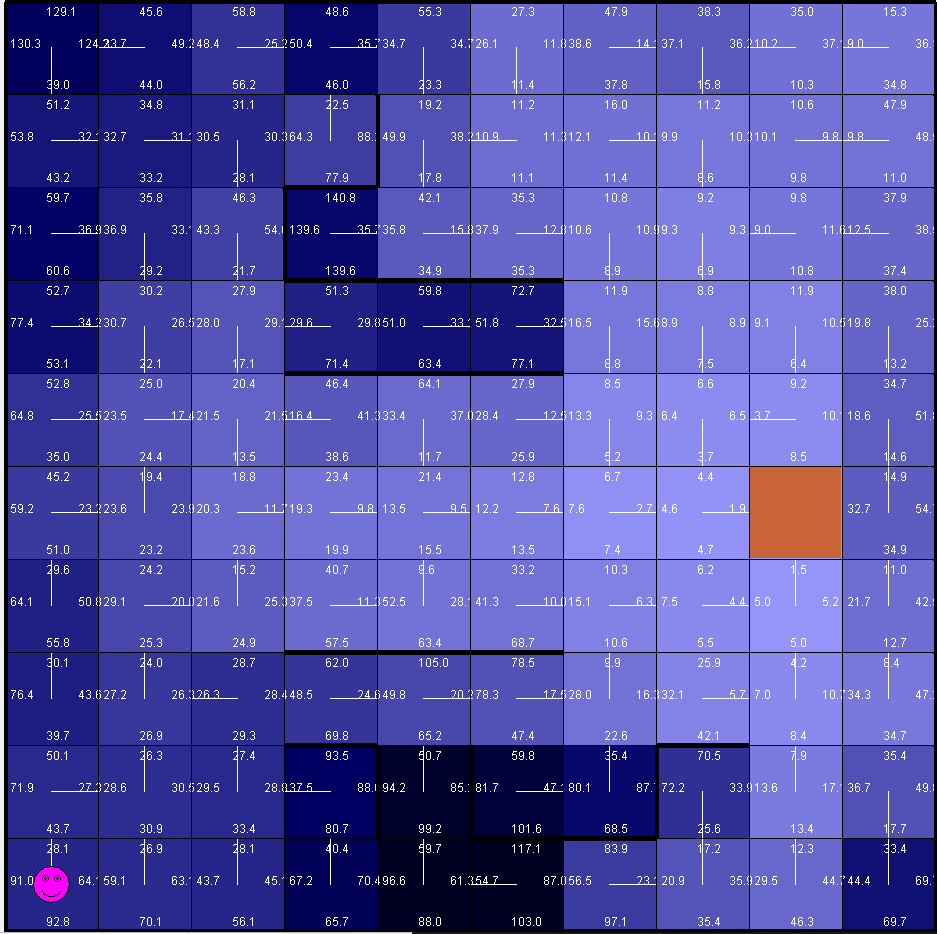
\includegraphics[width=5cm]{../images/small/q_1000.PNG}

            There were much more iterations done for Q-learning than
            for the other two algorithms, but the policy is less clear
            (as can be seen as the values here are not as dark, implying
            that the Q-learning agent has been trained much less). For example,
            consider the block that is at the fourth column from the left
            and on the second row from the top. This block is more lightly shaded,
            implying that the RL algorithm has less confidence about what the
            expected reward would be starting from that state. RL Sim did
            not include an option to run the algorithm until convergence,
            but it is obvious becuase of this difference in tile shadings
            that this Q-learning algorithm did not converge even after 1000
            entire iterations.

            The value iteration algorithm had only taken 61 steps to converge,
            each step which took $O(s^2)$ time. Each of the 1000 steps in the
            Q-learning algorithm took $O(s)$ time (a week lower bound on the
            time, since the agent initially travels much more since it is
            new to the environment).

            It makes sense that the Q-learning algorithm would take much longer to
            converge. Reinforcement learning algorithms have to undergo an exploration/exploitation
            tradeoff, which is not present in the MDP algorithms, since the MDP algorithms
            already have perfect information about the rewards and the transition functions.
            Thus, the reinforcement learning algorithms ended up taking a significantly
            longer time than the MDP algorithms. Even in the 10 x 10 maze, where
            the state space is quite small, there are still 100 total states and almost 400
            possible actions, which the agent meeds to try one at a time in order to achieve
            the information that an MDP has.

        \subsection{Maze: More States}

            Here is the image of the particular maze used for a large
            number of states. The end state is represented by the orange square.

            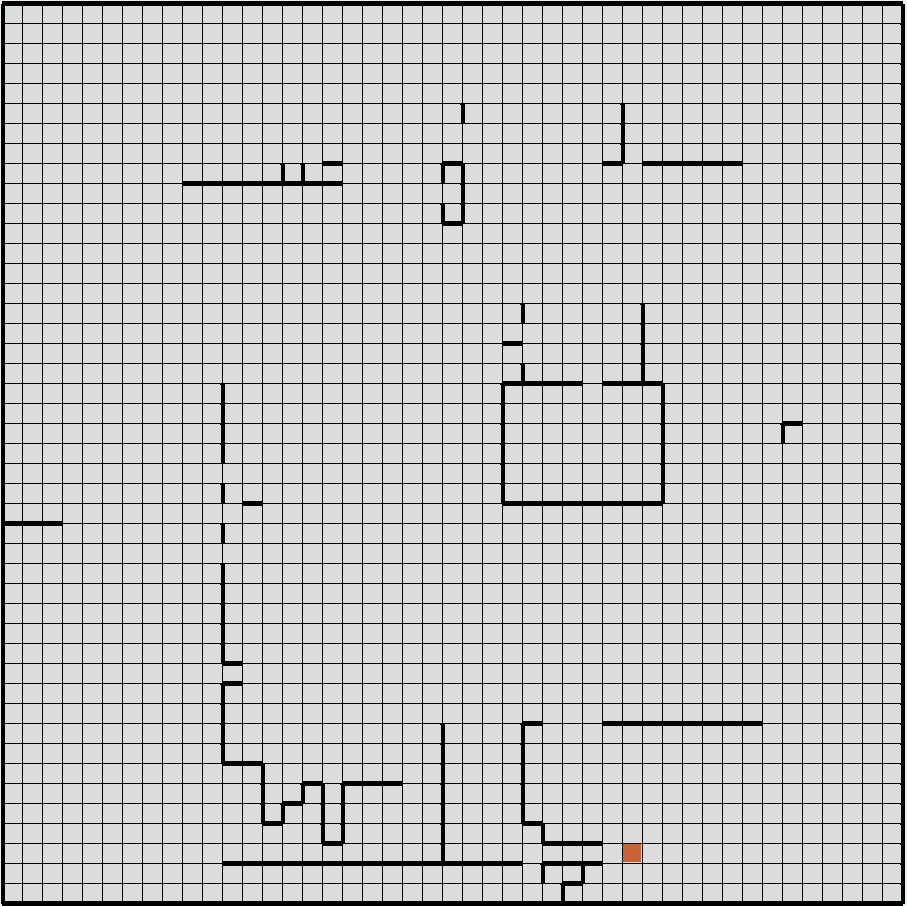
\includegraphics[width=5cm]{../images/large/maze.PNG}
            

            \subsubsection{Value iteration}

            %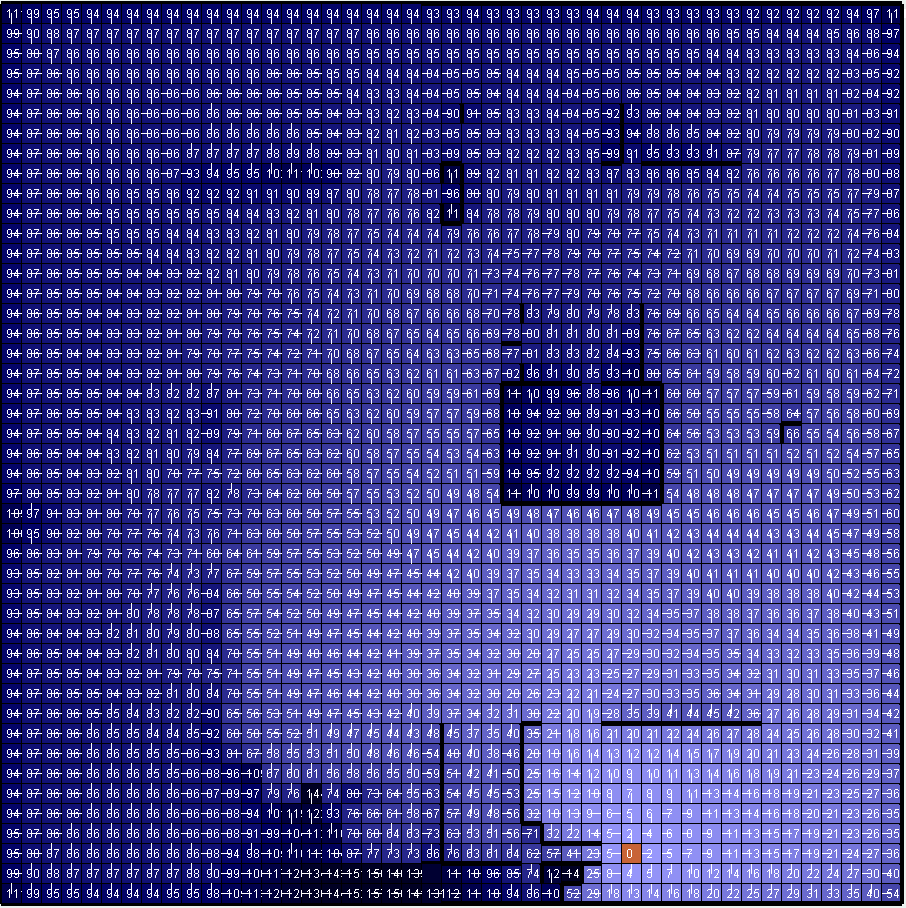
\includegraphics[width=5cm]{../images/large/vi_100.PNG}
            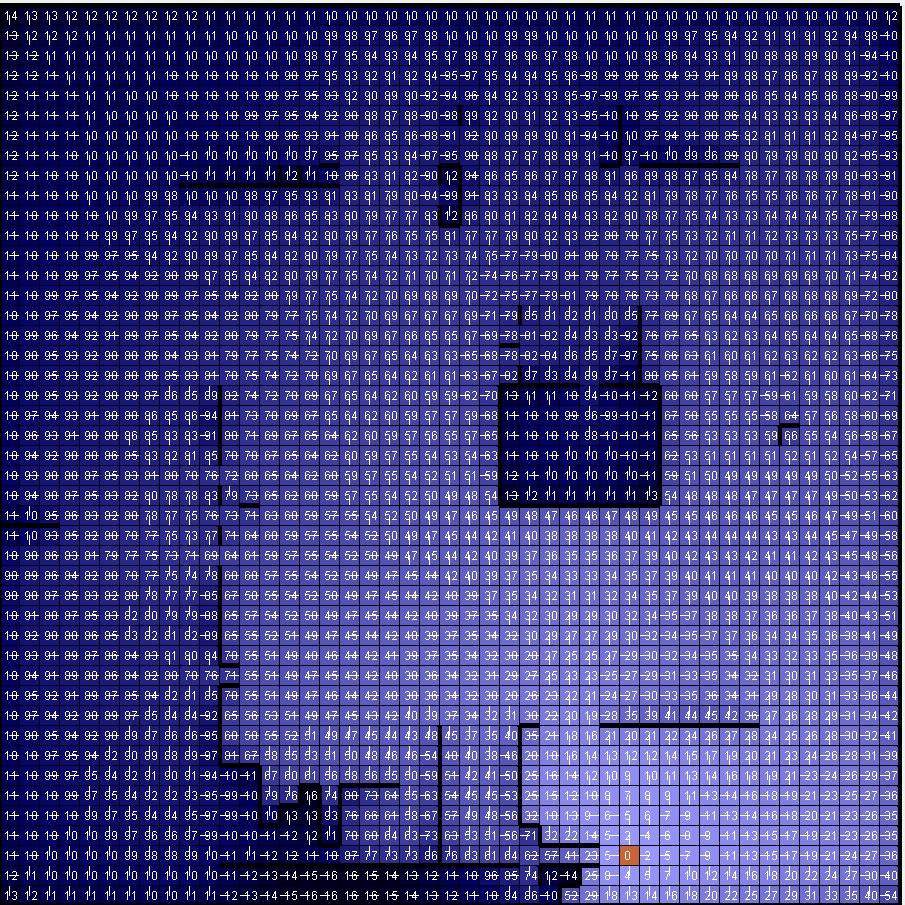
\includegraphics[width=8cm]{../images/large/vi.PNG}

            The image above is the final
            distribution of the values and policies

            The value iteration converged after 181 steps, and the algorithm
            took 10,871 ms.

            \subsubsection{Policy Iteration}

            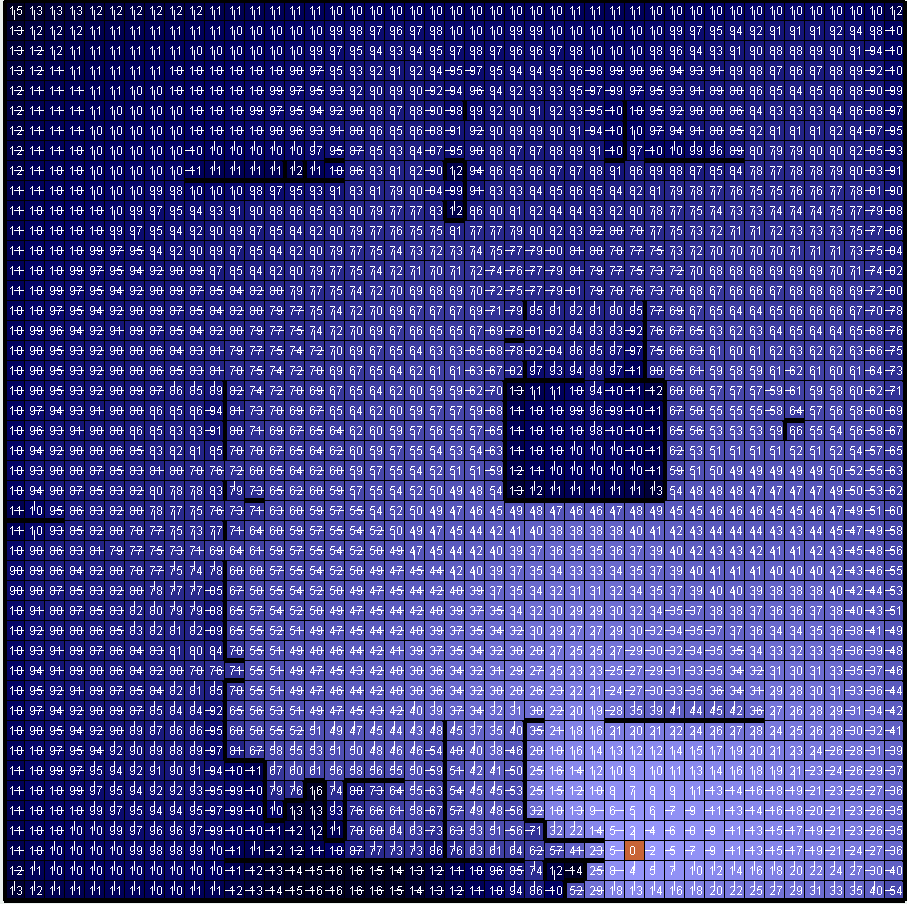
\includegraphics[width=5cm]{../images/large/pi.PNG}

            The policy iteration converged after 18 steps for 10 inner
            policy iterations, and the algorithm
            took 2,841 ms, which is much faster than the value iteration algorithm.

            However, using a smaller number of value updates for policy iteration here produces
            a different result when compared to using a smaller number of updates in the
            small maze, as shown below:

            \begin{tabular}{c c c}
                Inner iterations & Policy iterations & Time \\ \hline
                1 & 104 & 3516ms \\ \hline
                2 & 55 & 2908ms \\ \hline
                5 & 8 & 12ms \\ \hline
                10 & 18 & 2841ms \\ \hline

            \end{tabular}

            First of all, the number of policy iterations decrease as the number of inner iterations
            increases. This makes sense since there exist several squares that are very distant
            (at least 5 squares away) from any walls. Thus, for fewer inner iterations like one iteration,
            it takes multiple value updates for the information that a wall exists to propogate to certain
            squares; thus, more policy iterations are needed for fewer inner iterations.

            Also, the algorithm takes more time to run with fewer inner iterations, unlike what
            occurred with a smaller maze. Even though each policy iteration is faster due to
            fewer inner iterations, there are so many policy iterations that the total time
            is ultimately increased.
            
            Another reason for the longer runtime with fewer inner iterations is that there is a very large number of
            tiles, so more tiles are expected to be sensitive to noise due to action
            stochastisity. As explained previously,
            having fewer value updates causes certain policy estimates to be vulnerable to noise,
            so there would be a delay in the runtime of the algorithm.

            \subsubsection{RL}

            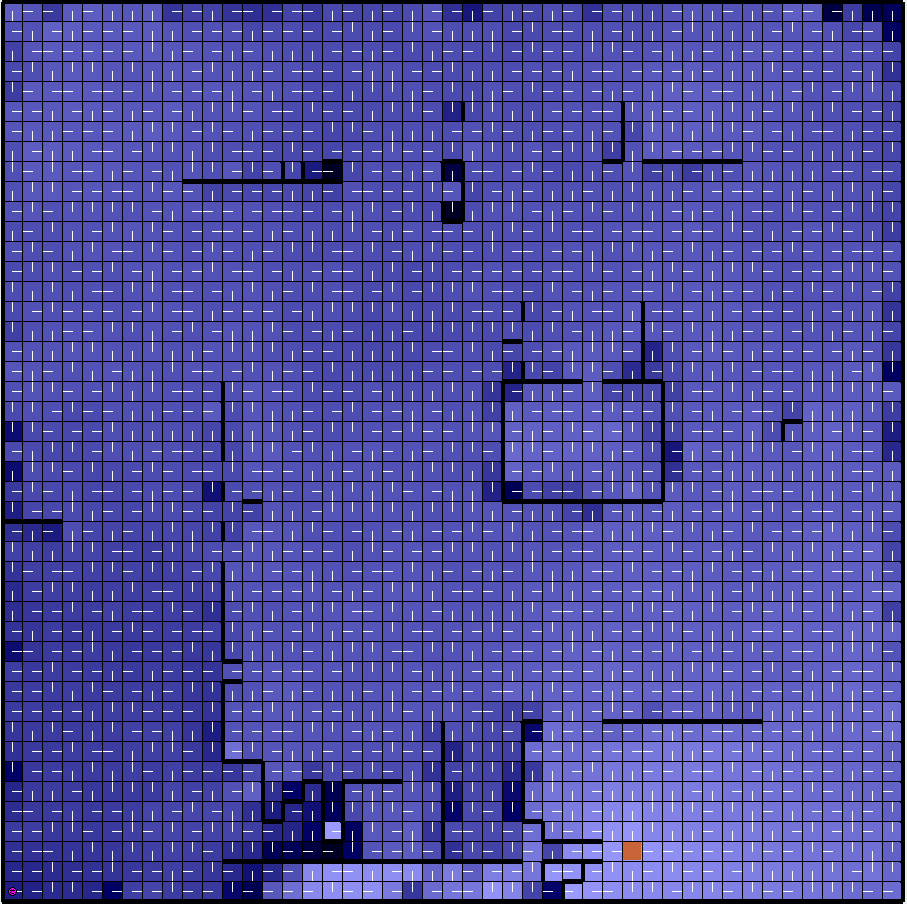
\includegraphics[width=8cm]{../images/large/q_20.PNG}
            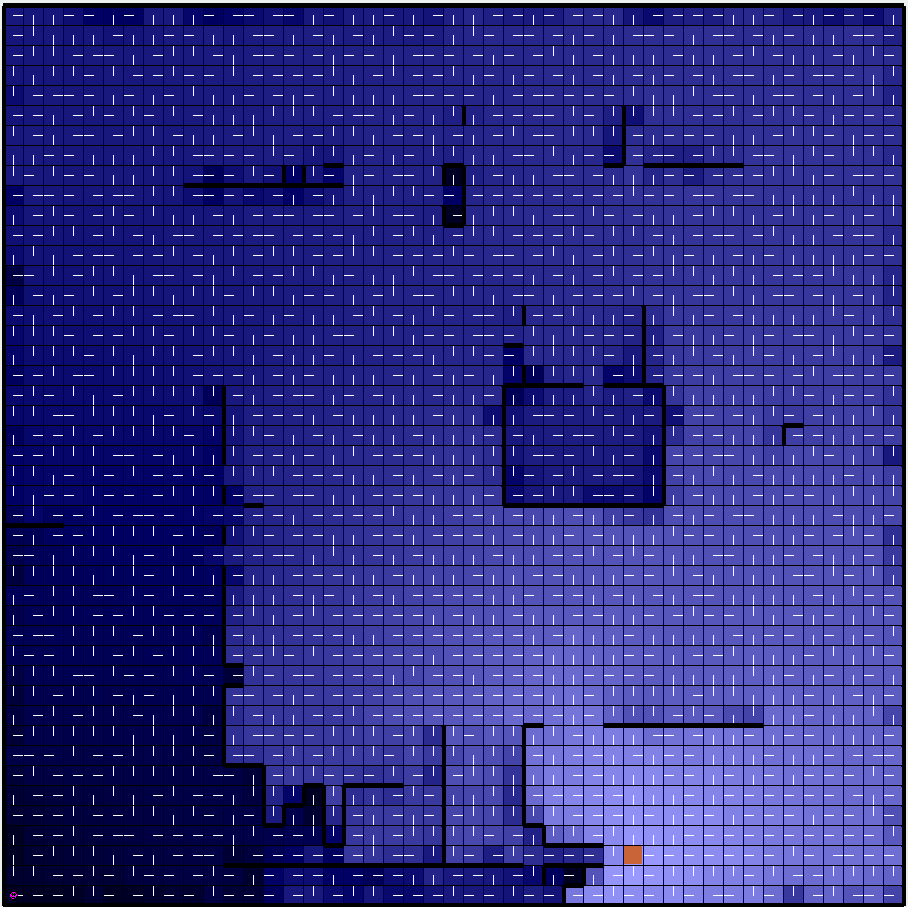
\includegraphics[width=8cm]{../images/large/q.PNG}

            The above images show the direction of the policy, and the shading
            of each tile represents the value at that tile. The image on the left
            shows the algorithm after 20 episodes, and the one on the right shows
            the completed algorithm after running for 1000 episodes.

            One trend that is noticeable is that the Q-learning algorithm has produced
            very accurate policies at the bottom left corner of the grid. Unlike in value
            iteration and policy iteration, the value tiles at the bottom left corner of
            the grid are very dark, indicating a strong confidence of the algorithm about
            what needs to be done from the states of that region to maximize the reward.

            However, even after 1000 cycles (which involves significantly more computations
            than policy iteration and value iteration, for similar reasoning as was
            mentioned in the discussion of the Q-learning algorithm for the smaller maze),
            the policies at the top right corner of the grid are very inconsistent
            with each other. Several
            of the tiles have policies that indicate that the optimal action is upward, but
            this is obviously not true.
        \section{Sources}
        
        [1] https://www.cs.cmu.edu/~awm/rlsim/

    \end{document}